\documentclass[11pt]{article}
\title {Oenone Scott CMEE MiniProject: Fitting models to functional response 
curves \\ Does the ratio of mass size of consumers and resources play a role in 
determing the most appropriate models to use}
\author{Oenone Scott}
\date{6 March 2020}
\usepackage{geometry}
\usepackage{graphicx}
\usepackage[]{lineno}
\usepackage[backend=biber,style=authoryear,bibencoding=utf8]{biblatex}
\usepackage{verbatim}
\usepackage{setspace}
\usepackage{array}
\usepackage{wrapfig}
%\usepackage{caption}
\newcolumntype{L}[1]{>{\raggedright\let\newline\\\arraybackslash\hspace{0pt}}p{#1}}
%\newcolumntype{C}[1]{>{\centering\let\newline\\\arraybackslash\hspace{0pt}}m{#1}}
%\newcolumntype{R}[1]{>{\raggedleft\let\newline\\\arraybackslash\hspace{0pt}}m{#1}}

\doublespacing

% Word Count command %
\newcommand\wordcount{\input{../Code/thesisWordcount.sum}}	



% bibliography section %

\addbibresource{thesisRef.bib}



\begin{document}

\begin{titlepage}


	\centering % this centers everything on the page
		
	%\vspace  % Whitespace at the top of the page 
	
	
	% --------------------------
	%% TITLE
	
	\vspace*{3\baselineskip}
	
	\rule{\textwidth}{1.6pt}\vspace*{-\baselineskip}\vspace*{2pt} % Thick horizontal rule
	\rule{\textwidth}{0.4pt} % Thin horizontal rule
	
	\vspace{0.75\baselineskip} % Whitespace above the title
	
	{\LARGE FISH ARE THE BEST  \\} 
	
	\vspace{0.75\baselineskip} % Whitespace below the title
	
	\rule{\textwidth}{0.4pt}\vspace*{-\baselineskip}\vspace{3.2pt} 
	\rule{\textwidth}{1.6pt} 
	
	\vspace{2\baselineskip} 
	
	% ---------------------------------
	%% SUPERVISORS & CONTACT EMAIL
	
	Word count: 	
	\wordcount words
		
	\vspace{0.5 \baselineskip} % Whitespace between text
	

	Scott, Oenone. \\
	
	Contact: ojs19@imperial.ac.uk
	
	\vspace*{1\baselineskip}
	
	A thesis submitted in partial fulfilment of the requirements for the 
	Computational Methods in Ecology and Evolution Master of Research at 
	Imperial College London \\
	Formatted in the Harvard Style \\

\end{titlepage}

\linenumbers

\section{Abstract}
\noindent


	
	\section{Introduction}
	\noindent

\subsection{The need for conservation efforts }
Our planet is currently losing species at such a significant rate that this 
period has been called the "Sixth mass extinction" 
\autocite{Barnosky2011}. There are many valid reasons as to why this is viewed 
as a negative thing; these range from losing 'ecosystem services'- i.e. we 
humans will lose valuable future sources of medicine and food, to the 
intrinsic value that having biodiverse ecosystems have, which is harder to 
quantify. True extinction events cannot be reversed (sorry, Jurrasic Park), but 
through conservation action, species that are extinct in the wild can be 
reintroduced; vulnerable or threatened species can be protected, and entire 
ecosystems can be protected. Unfortunately, conservation actions are be 
resource intensive and can be expenive, and we are unable to protect every 
threatened or 
vulnerable species on the planet - and this is compounded by the fact that we 
do not have comprehensive, up-to-date data on which species are threatened 
globally. Therefore, with the knowledge that we do have, conservationists are 
being forced to select which species to prioritise. There are many metrics by 
which conservationists evaluate species' worthiness of protection, and the 
methods through which they can be best conserved. Some metrics focus on a 
species' "irreplacabilitiy" (i.e. focus on endemic species); others focus on 
physiological or genetic 'uniqueness', unusual abilities, or species living in 
rare habitats \autocite{Brooks2006}. The problem with some of these approaches 
is that they can be skewed towards organisms that are charismatic (i.e. the 
Giant Panda), and miss species that are small, visually unremarkable, or that 
may be the sole survivor of millions of years of evolutionary history 
\autocite{Clark2002}. There is significant taxonomic and geographic bias 
reported in conservation research \autocite{Clark2002, Darwall2011, 
Watson2017}, which highlights the clear need for a quantitative, universally 
applicable method of determining species which require conservation 
prioritisation.  The 
'EDGE' metric seeks to solve this problem of biased prioritisation by 
considering only the evolutionary history represented by species, and it's 
level of endangeredness. It is calculated by combining a species 'Evolutionary 
Distinct' (ED) score, with it's 'Global 
Endangered' score (EG). A species' ED score is calculated using a phylogenetic 
tree, and the score represents the numbers of millions of years of evolutionary 
history that is within that species \autocite{Isaac2007}. Species that have 
speciated recently, or that have many recent 'cousin' species will have lower 
ED scores than species that have no close living relatives, and that speciated 
a long time ago. 

\begin{wrapfigure}{t}{0.5\textwidth}
	
	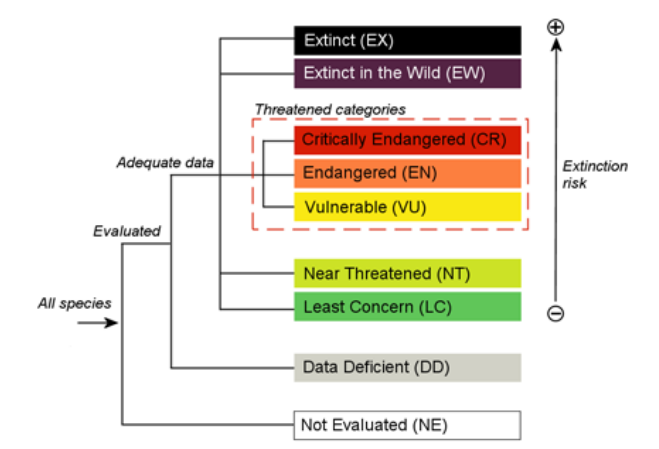
\includegraphics[width=0.35\textwidth]{Images/RedListCategories.png}
	\caption{IUCN Red List categories}
	\caption{ \autocite{IUCN2000}})
	\label{IUCNcategories}
	
\end{wrapfigure}

The GE score of a species is calculated using the IUCN's 'Red 
List' assessment for that species \autocite{Isaac2007}, in which species are 
categorised according to how stable their populations are and how likely they 
are to become extinct \autocite{IUCN2000}. These categories are shown in Figure 
~\ref{IUCNcategories}. This metric was chosen for this 
study as it provides a mechanism to comprehensively assess species with family 
groups (or larger), and this study believes it will produce results that can be 
used to meaningfully influences the manner in which these species are 
considered. 

\subsection{Why fish?}

The group considered in this study are the \(Actinopterygii\), commonly 
known as the ray-finned fish. Actinopterygii are the largest class of 
vertebrate, with over 33,000 constituent species \autocite{Fishbase}. Fo 
context, mammals are thought to have closer to 6,400 extant species 
\autocite{Mammal2020}; reptiles have 9,500 species 
\autocite{Pincheira-Donoso2013}
; and birds have around 18,000 \autocite{Barrowclough2016}. Unfortunately, the 
Actinopterygii are also proportionally 
the most understudied classes of the vertebrates, with just over 50\% assessed, 
compared with the 62-90\% of other classes, as laid out in 
Table ~\ref{ClassAssessment}. \\

	\begin{tabular}{lrrr}
	\textsc{Class} & \textsc{\# of Species} & \textsc{\# Assessed} & \textsc{\% 
	Assessed} \\	
	\hline
	\textsc{Actinopterygii}	& 33,000 & 17,955 & 54.4 \\
	\textsc{Mammalia} & 6,500 & 5850 & 90.0 \\
	\textsc{Aves} & 18,000 & 11,147 & 62.0 \\
	\textsc{Reptilia} & 9,400 & 7892 & 84.0 \\ 
	\multicolumn{4}{l}{\caption{Table ~\ref{ClassAssessment}: IUCN 
	Red List  assessments for vertebrate classes}} \\
	\multicolumn{4}{l}{ \autocite{Mammal2020, Pincheira-Donoso2013}} \\
	\multicolumn{4}{l}{ \autocite{Barrowclough2016, Fishbase}}
	\label{ClassAssessment}
	
\end{tabular}
\newline
\newline

The IUCN is not the only research body in which Actinopterygii are poorly 
represented. A 
quick search in WebofScience also demonstrates the lack of research into this 
class. When searching for topics that include the class names of the groups 
mentioned in Table ~\ref{ClassAssessment}, the results are as follows: 
Actinopterygii -2055; Mammalia - 8905; Reptilia - 6,030; Aves - 13,116.

Despite the lack of studies into Actinopterygii, many species of fish are 
acknowledged to be very important as a source of food and employment - through 
fishing, harvesting activities and tourism and entertainment. Fish consumption 
has been rising steadily for the past 6 decades, as highlighted clearly in 
Figure ~\ref{GlobalCatch}. 

\begin{wrapfigure}{r}{0.4\textwidth}
	
	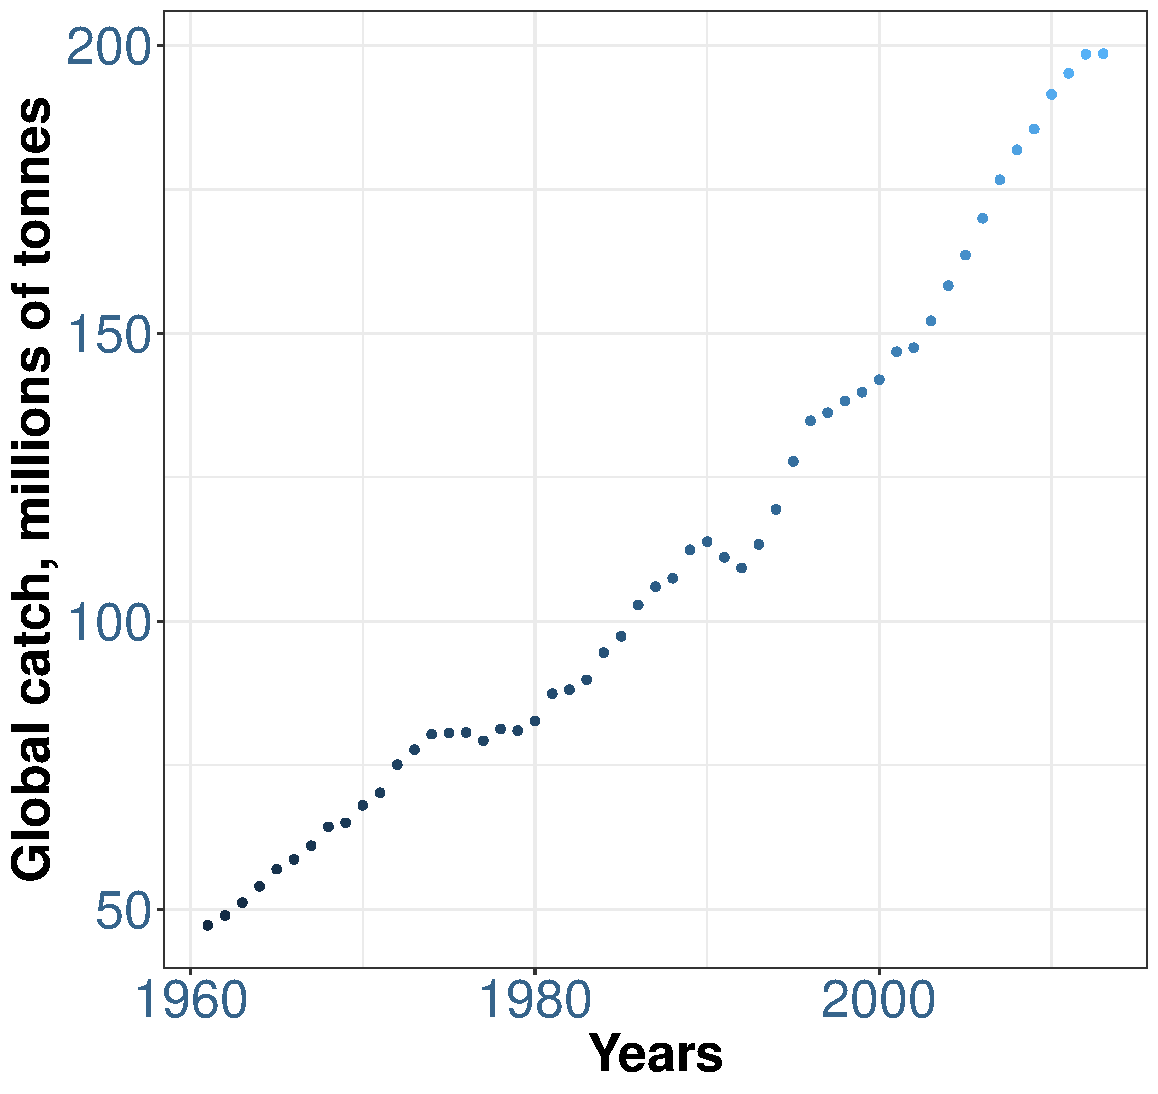
\includegraphics[width=0.35\textwidth]{Images/GobalCatch.pdf}	
	\caption{Global catch of marine fish, in millions of tonnes \\
	\autocite{FAO2020} }  
	\label{GlobalCatch}
	
\end{wrapfigure}


Many people, especially in Europe and Northern 
America, are increasing the amount of fish in their diet - some due to 'health 
reasons'(eating fish is documented to beneficial to human health 
\autocite{Rimm2006}), and others to 
lessen their impact on the environment \autocite{Mary2020}. Younger generations 
are particularly aware of the impact their food choices have on the planet 
\autocite{Mary2020}, so it could be assumed that this trend of eating more fish 
is unlikely to change. This increased demand for fish (and fish-related 
products) has lead to an increase in aquaculture (farming fish) 
\autocite{Belton2018}. Wild-caught 
fish number are in decline due to stock exhaustion and 
populating collapse rather than a decrease in interest in wild caught fish 
\autocite{Tremblay2011, Belton2018}. 

Marine ecosystems in particular are under increasing pressure from human 
action. Globally, governments and scientific bodies have agreed that ecosystems 
need to be protected in order to protect the future of marine resources 
\autocite{MurakiGottlieb2018}. Marine Protected Areas (MPAs) are one form of 
protection - 
however the definition of these vary significantly from one location to 
another \autocite{Marinesque2012}. In general,  a MPA's success is evaluated by 
its effectiveness at conserving 'keystone' species, or their value to local 
fishing activities \autocite{Marinesque2012}. As discussed above, by 
considering only 'keystone' species, considerable ecosystem damage may occur 
un-measured, and diverse species. 

Given that many species of fish 
exist in both the marine and freshwater realms, and many more migrate around 
the globe, clear conservation priotisiation for fish will be crucial to ensure 
we do not fail to protect vulerable and non-charismatic species. 


\subsection{X, Y  and Z}
subsection: why these fish in particular



It is clear that the Actinopterygii group is both under-studied and 
under-protected, despite their importance to human populations across the 
globe. This study is a first step in directly addressing this imbalance. Using 
the EDGE metric, we create conservation prioritisation lists for [X, Y and Z] 
and, along with geospatial analysis of their current habitats and threats, 
highlight methods through which vulnerable species could be protected. This 
study also provides a roadmap that will be useful for the creation of reports 
regarding other family groups within the Actiopterygii class.  






	\section{Methods}
	\noindent




\section{Results}
\noindent




\section{Discussion}
\noindent



%	\section{References}
\noindent
\printbibliography 


\section{Appendix 1: Figures}

	



\end{document}